The standard model is arguably the most successful theory in all of physics.
It uses the language of quantum field theory to describe the elementary particles of the universe and their interactions via the electromagnetic, weak, and strong forces.
\autoref{fig:the standard model} shows a table of the particles that make up the standard model.
Calculations of observable quantities using quantum electrodynamics (QED), the quantum theory of electromagnetic interactions, and the theory of weak interactions give highly precise predictions which agree to an astounding degree with experiments~\cite{Schwartz:QFT}.
These calculations use the techniques of Feynman diagrams, which describe any interactions as the sum of all possible ways that interaction could happen.
When the interaction is weak, as is the case for QED, we get a sum that converges quickly, and calculating a few orders of the sum will yield highly accurate estimates of physical quantities.
The weakness of QED is quantified in the fine structure constant $\alpha \approx 0.00 7297$~\cite{PDG}.
A Feynman diagram in QED is proportional to $\alpha^n$, where $n$ is the number of vertices in the diagram.
\todo{Is this really how Feynman diagrams work? Are they actually asynmptotic series?}
Consequently, the contributions from more complex diagrams with many vertices rapidly become insignificant.
Feynman diagrams are illustrated in \autoref{fig:qed feynman diagrams}, where the first few diagrams in electron scattering are drawn.

\begin{figure}[h]
    \centering
    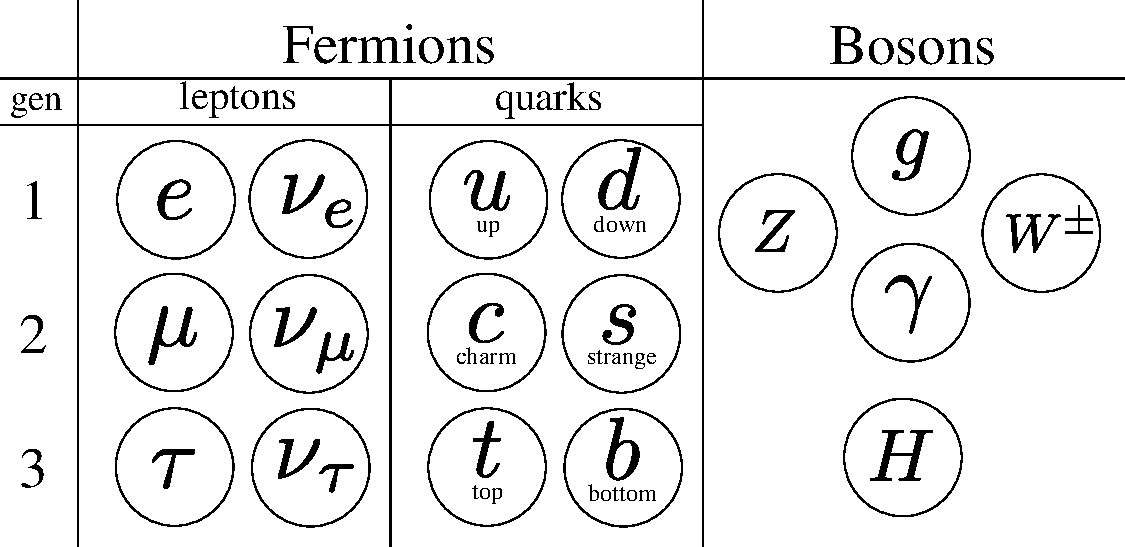
\includegraphics[width=0.7\textwidth]{figurer/standard_model2.pdf}
    \caption{The particles of the standard model. The fermions are made up of two leptons and two quarks in each generation, with three generations. The photon ($\gamma$) is the particle of the electromagnetic force, the gluon (g) of the strong force, and the $Z$ and $W^\pm$ bosons are responsible for the weak force. The final piece of the puzzle is the Higgs boson (H).}
    \label{fig:the standard model}
\end{figure}

Quantum chromodynamics, or QCD, is the part of the standard model that describes quarks, the constituents of protons and neutrons, and how they interact via the strong nuclear force.
When dealing with the strong force, the fact that the strength of interaction depends on the energy scale becomes apparent.
This dependence is due to what is called the \emph{running} of the coupling constant.
In high energy interactions at the energy scale of the $Z$-boson, $m_z \approx 91.19 \, \text{GeV}$, the strong force equivalent to the fine structure constant is $\alpha_s(m_Z) \approx 0.118$~\cite{PDG}. 
This makes it possible to do perturbative calculations using QCD.
However, the strong force has its name for a reason.
For scales around $1\, \text{GeV}$ and below, the perturbation method breaks down.
In this case, quarks bond together and form \emph{hadrons}.
Hadrons are classified as \emph{mesons} or \emph{baryons}.
The most familiar of the baryons are the proton and neutrons.
None of the mesons are stable, but they play an essential role in describing the strong force in the non-perturbative regime.
This is done by using \emph{effective field theories}, which we will cover in the next subsection.

\begin{figure}[h]
    \centering
    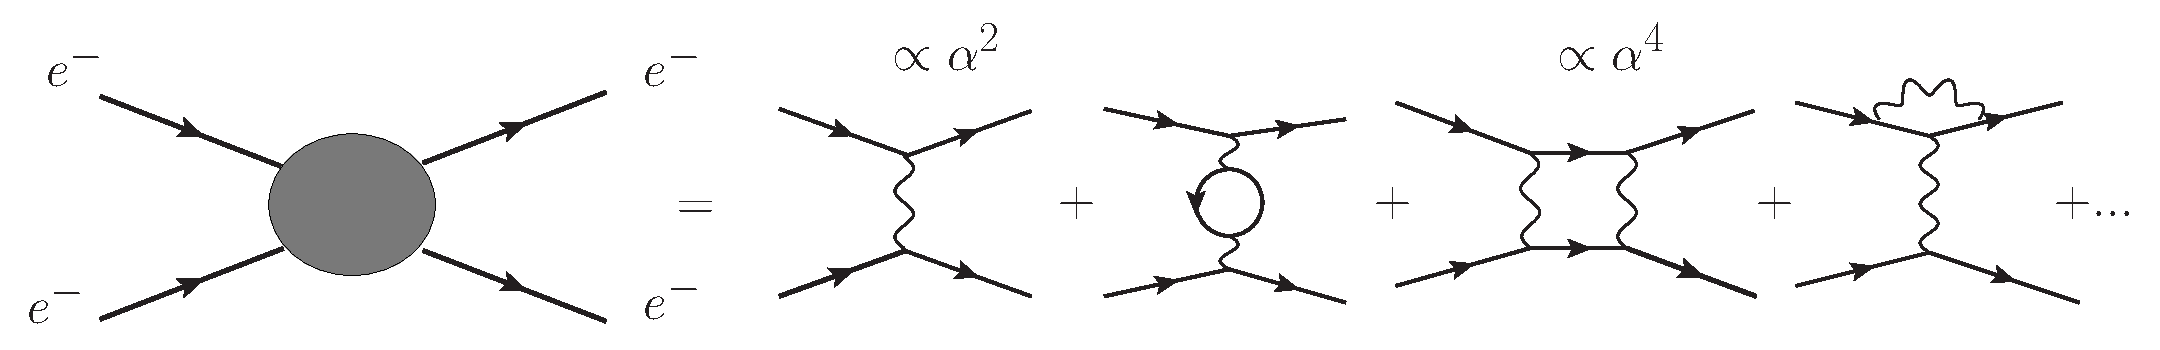
\includegraphics[width=0.95\textwidth]{figurer/feynman-diagram/sum_qed.eps}
    \caption{The process of electron scattering is described by the summation of Feynman diagramms representing all possible ways for the electrons to interact. Higher order terms are less important, as they pick up more and more powers of $\alpha$.}
    \label{fig:qed feynman diagrams}
\end{figure}

Mesons, of which pions are the lightest, were first proposed by Hideki Yukawa as the mechanism to hold nucleons together to form the nucleus of atoms.
Though first believed to appear in the showers of particles created by cosmic rays, they were decisively discovered in 1947 by Cecil F. Powell \emph{et al.}~\cite{griffiths:introduction}.
Pions do not show up in the standard model, as quarks do, but rather as an effective degree of freedom at low energy.


\subsection*{Effective field theories}

A profound feature of physics is the possibility of describing a system by isolating the degrees of freedom of interest, ignoring the rest.
We can describe the motion of the planets in the solar system, massive and complex systems, by only their mass, velocity, and position.
In quantum field theory, this feature manifests in the power of effective field theory.
An effective field theory describes a system not by the fundamental, underlying particles but by effective degrees of freedom.
A theory of two interacting fields $\varphi$ and $\psi$ will be described by an action that depends on both fields, $S[\varphi, \psi]$.
In the path integral formalism, predictions can then be made by integrating over all possible states of the fields.
An example is the vacuum transition amplitude,
\begin{equation}
    Z = \int \D \varphi \D \psi \, \exp{i S[\varphi, \psi]}.
\end{equation}
The effective description of only the $\varphi$-degrees of freedom by \emph{integrating out} the $\psi$-degrees of freedom, which results in an effective action $S_\text{eff}[\varphi]$, related to the underlying theory by~\cite{Schwartz:QFT}
\begin{equation}
    \label{integrating out degrees of freedom}
    \int D \varphi \, \exp{i S_\text{eff}[\varphi]} 
    =
    \int \D \varphi \D \psi \, \exp{i S[\varphi, \psi]}.
\end{equation}
This gives us hope for describing low-energy QCD as an effective theory of the particles we know from experiments appear.
In this specialization project, we will derive and explore chiral perturbation theory (\chpt), a low-energy effective theory of QCD where mesons are the degrees of freedom.

The action of the standard model has the form of an integral over a local Lagrangian,
\begin{equation}
    S[\varphi] = \int \dd^4 x \, \Ell[\varphi],
\end{equation}
where $\varphi$ denotes all fundamental particles.
The locality of $\Ell$ means that it is made up of terms like $\varphi(x) \varphi(x)$, where all interactions happen at one point in space-time, as opposed to a term such as $f(x, y)\varphi(x) \varphi(y)$.
We can not a priori expect an effective action to take this form~\cite{Schwartz:QFT}.
However, we have general principles we expect particles to obey, such Lorentz invariance and cluster decomposition.
Cluster decomposition concerns a system of $N$ sets of particles, $\alpha_i$, that evolve into the sets $\beta_i$.
That is,
\begin{equation}
    \ket{\alpha_1, \alpha_2, ... \alpha_N}_\text{in}
    \longrightarrow
    \ket{\beta_1, \beta_2, ... \beta_N}_\text{out}.
\end{equation}
It says that if the sets of particles $\alpha_i$, $\beta_i$ are located far enough apart, then the $S$-matrix factors as
\begin{equation}
    {\braket{\beta_1, \beta_2, ... \beta_N}{\alpha_1, \alpha_2, ... \alpha_N}}
    =
    \braket{\beta_1}{\alpha_1}\braket{\beta_2}{\alpha_2}... \braket{\beta_N}{\alpha_N}.
\end{equation}
This is a familiar property, as it essentially says that wildly separated experiments do not interfere, and one that we expect all good effective descriptions to have~\cite{weinberg_1995,weinberg_1996_vol2}.
These principles greatly constrain any effective action and are the basis for constructing the \chpt\, effective action.
This method was formulated by Weinberg~\cite{WeinbergPhenom} 
It relies on---as Weinberg himself called it---a ``theorem'':
\begin{quote}
    ``[I]f one writes down the most general possible Lagrangian, including all terms consistent with assumed symmetry principles, and then calculates matrix elements with this Lagrangian to any given order of perturbation theory, the result will simply be the most general possible $S$-matrix consistent with analyticity, perturbative unitary, cluster decomposition and the assumed symmetry principles.'' \cite{WeinbergPhenom}
\end{quote}
In other words, if we write down the most general Lagrangian consistent with symmetries of the underlying theory, then we have not made any restrictions on the theory, other than some foundational assumptions.
This Lagrangian will be of the form
\begin{equation}
    \Ell_\text{eff}[\varphi] = \sum_i \lambda_i \mathcal O_i,
\end{equation}
where $\mathcal O_i$ are local functions of the fields and their derivatives, and $\lambda_i$ are coupling constants.
The coupling constants are free parameters, which parametrizes the most general $S$-matrix consistent with foundational assumptions and the underlying theory.
A Lagrangian with an infinite amount of free parameters might seem useless. 
However, if we can find a consistent series expansion, then only a finite number of terms are needed to calculate quantities to any given order in perturbation theory.
In the case of \chpt, the expansion is in the momentum of the pions.
We will detail this later in the text.


\subsection*{Stars}

Although it might seem counterintuitive, stars are one of the objects we might hope to describe using QCD at low energies.
Neutron stars, one of the most extreme objects in the universe, quickly cool down to temperatures below $10^{10} \, \text{K}$.
This might be hot by almost all standards. 
However it corresponds to an energy of $0.862 \, \text{MeV}$.
This is well below the perturbative regime of QCD, and the stars must therefore be described by an effective model of interacting nuclear matter~\cite{glendenning:compcat_stars,from_hadrons_to_quarks}.
Stars are modeled using the Tolman-Oppenheimer-Volkoff, or TOV, equations.
The TOV equations are based on Einstein's general theory of relativity, and its solution gives the star's pressure as a function of its radius.
The only input needed is the \emph{equation of state}, or EOS, of the matter that makes up the star~\cite{Carroll:spacetime}.
The equation of state of a matter is the relationship between its energy density, $u$, and pressure $P$, i.e. a relationship of the form
\begin{equation}
    f(P, u) = 0.
\end{equation}
This is where QCD comes in.
One way to compute the equation of state of QCD systems is using the numerical method called lattice QCD.
Here, space-time is approximated as finite and discrete, and Monte-Carlo importance sampling is used to perform the path integral.
This method, however, fails for non-zero baryon chemical potential $\mu_B$, in what is known as the fermion sign problem.
The baryon chemical potential $\mu_B$ parametrizes the matter-antimatter asymmetry.
There is much more matter than antimatter in neutron stars, or more generally, all observed stars.
This makes lattice QCD unsuited for simulating these systems.
Recently, it has been proposed that a condensate of pions can form a new type of compact, gravitationally bound object, i.e., a star.
States of pion condensates can have zero baryon chemical potential and are thus amenable to lattice QCD simulations.
This offers a way to model stellar objects from first principles, as well as by analytical methods using \chpt~\cite{new_clas_of_compact_stars,andersen:bose_einstein}.

\subsection*{Pion condensate and the QCD phase diagram}

In addition to their electrical charge, the pions have an \emph{isospin} quantum number, $I_3 = -1, 0$ or $1$.
There is also a corresponding isospin chemical potential $\mu_I$, which parametrizes how much the system favors a negative of positive isospin charge.
In a pion condensate, the system has a non-zero isospin density $n_I$.
This condensation happens when the isospin chemical potential reaches a critical value, $\mu_I = \mu_I^c$.
The pion condensate is an expample of Bose-Einstein condensation, in which a macroscopic number of bosons occupy a single quantum state~\cite{Brandt:QCD_phase_diagram_with_isospin_chemical_potential,Brandt:QCD_phase_diagram_for_nonzero_isospin-asymmetry}.

The pion condensate phase is just one part of the rich phase structure of QCD, which is an active field of research.
In \autoref{fig:phase diag qcd}, we show a rough sketch of the phase diagram of QCD.
We emphasize that the understanding of this diagram is far from complete.
The difficulties of exploring QCD, such as the non-perturbativity at low temperatures and the fermion sign problem mentioned in this text, means that much of the phase diagram is only conjectured.
At low temperatures and chemical potentials, in the so-called normal or vacuum phase, we get a hadronic gas.
This corresponds to all but the most extreme situations.
\todo{Be more exact. High temp. and c.p. is not the same.}
For high temperature or chemical potentials, QCD-matter undergoes \emph{deconfinment}, as the strong force weakens due to the running of the coupling constant.
In this phase, quarks are no longer tightly bound in hadrons, but together with gluons, form a soup called \emph{quark-gluon plasma}.
Observations of a non-hadronic state of QCD-matter were done at the Relativistic Heavy Ion Collider (RHIC) in 2005~\cite{2005:RHIC,2005:RHIC2}.
Quark gluon plasma is conjectured to be present at the center of neutron stars~\cite{from_hadrons_to_quarks}.
A color superconductor is believed to form at low temperatures and high baryon densities, which corresponds to high baryon chemical potentials.
This state of matter is analogous to electrical superconductors, in which electrons form Cooper pairs allowing for unimpeded electrical current.
The color superconducting phase is due to the forming of Cooper pairs of quarks and results in the Meissner effect in which gluons can acquire mass~\cite{alford:color_superconductivity}.

Understanding the phase diagram of QCD is an important part of research into the standard model and its consequences.
It is essential to use all possible sound approaches to validate the techniques used.
This allows for validation of methods by comparing results in the overlapping regimes, such as when comparing \chpt\ with lattice QCD.

\begin{figure}[h]
    \centering
    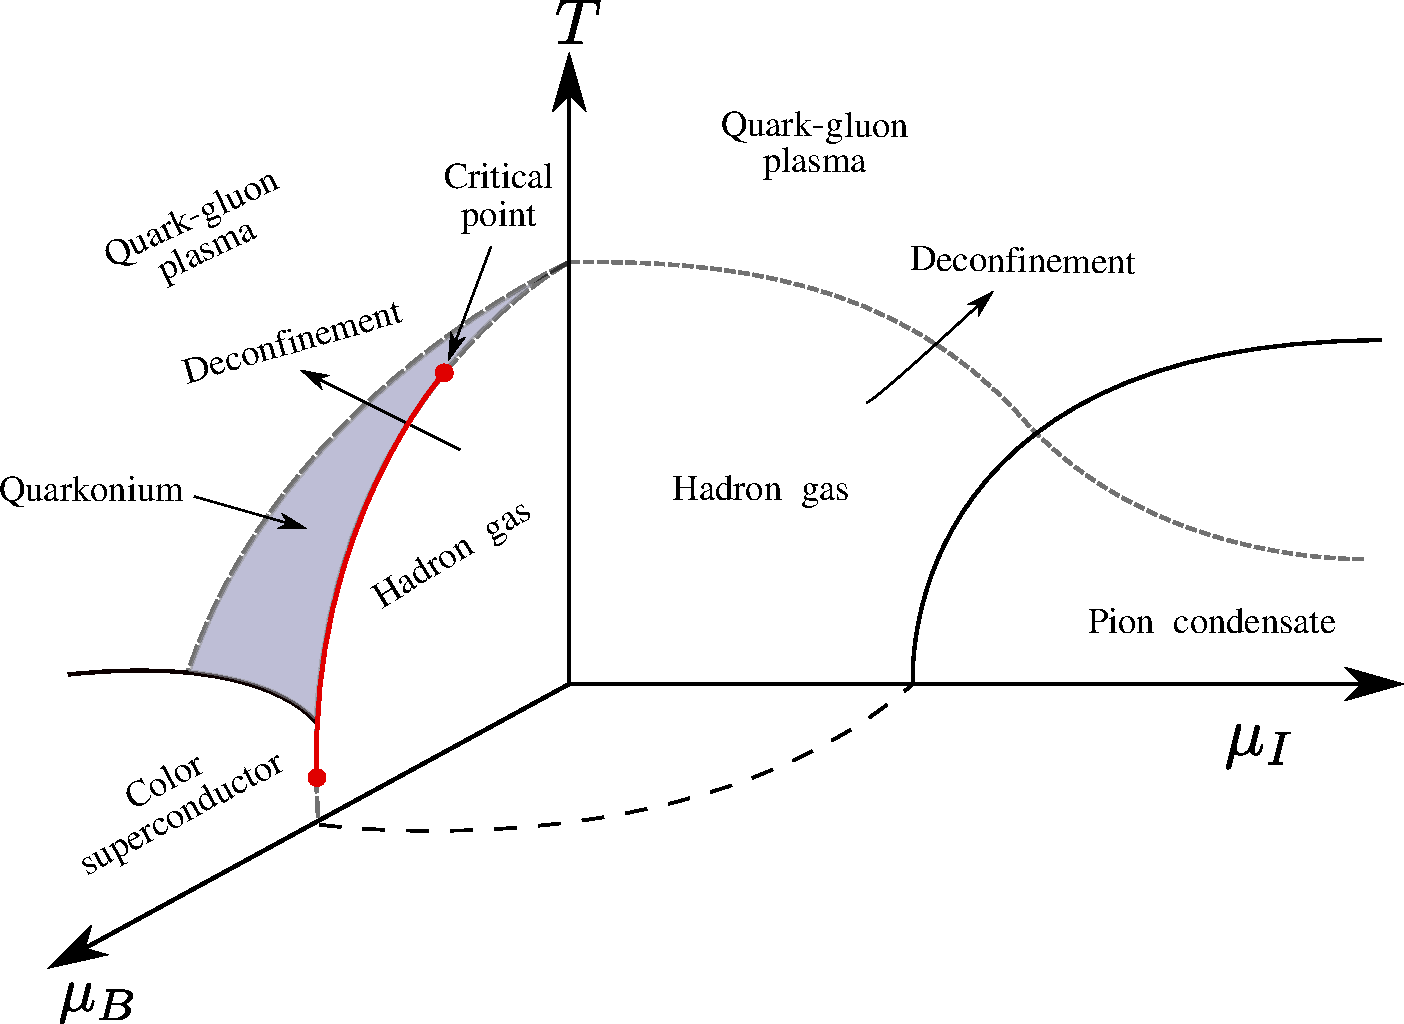
\includegraphics[width=0.9\textwidth]{figurer/phase_diagram2.pdf}
    \caption{A sketch scetch of the phase diagram of QCD. See text for description. Based on~\cite{from_hadrons_to_quarks,
    Brandt:QCD_phase_diagram_with_isospin_chemical_potential,Brandt:QCD_phase_diagram_for_nonzero_isospin-asymmetry,Fukushima:The_phase_diagram_of_dense_QCD,mannarelli:meson_condensation}
    }
    \label{fig:phase diag qcd}
\end{figure}

\subsection*{Outline of thesis}
This thesis aims to calculate the next-to-leading order equation of state of a system at finite isospin chemical potential, using two-flavor chiral perturbation theory.
We will also investigate the phase transition from the vacuum phase into a pion condensate phase.
In \autoref{chapter:theory}, we take a survey of some general theory needed for \chpt.
We introduce the generating functional in the path integral formalism and use this to define the one-particle-irreducible effective action and the effective potential.
This allows us to prove Goldstone's theorem, an important result that provides the connection between the symmetries of a theory and its low energy dynamics.
The theorem states that spontaneous symmetry breaking gives rise to massless particles.
We then present the CCWZ construction, which provides a procedure to construct an effective Lagrangian of Goldstone bosons.
We also present some mathematical prerequisites, such as Lie groups and Lie algebras, and discuss the role and mathematical implementation of symmetries in physics in general and quantum field theory in particular.

In \autoref{chapter:effective theory of pions}, we take the general theory of the last chapter and apply it to QCD to get \chpt.
We start the chapter by discussing QCD, its constituent parts, symmetries, and the corresponding conserved currents.
We then use the theory from the last chapter to find the terms that make up the Lagrangian of \chpt and how to incorporate explicit symmetry breaking, external source currents, and a finite isospin chemical potential.
This section also contains a discussion about how to order these terms in a well-defined series expansion and avoid the need to include infinity many terms.
With this, we construct the leading order and next-to-leading order Lagrangian, which is expanded in powers of the pion fields.
We discuss how to identify possible redundant terms in the Lagrangian and use our result to find properties of the pion, such as their tree-level mass and propagator.

\cref{chapter:thermodynamics} is dedicated to the thermodynamic properties of \chpt.
We use the derived Lagrangian to calculate the free energy density to one loop using the leading order Lagrangian. 
Then, we use the tree level free energy density at next-to-leading order to renormalize the result.
We discuss the low energy parameters we use and consistently evaluate observable to the same order in the series expansion.
With the free energy density, we derive the equation of state at finite isospin chemical potential.
We also discuss the phase transition to the pion condensate phase using the Landau theory of phase transition.

We summarize the results and discuss further work in \autoref{chpater:conclusion and outlook}.
The appendix is referenced throughout the text.
In \autoref{appendix:thermal field theory}, we review thermal field theory and the imaginary time formalism.
This chapter contains calculations needed in the central part of the thesis, where they are referenced, and lays out the path integral approach and its connection to thermodynamics in more detail.
We also discuss dimensional regularization, derive the Feynman rules for and interacting scalar, and generalize thermal field theory to fermions.
The other appendices discuss some mathematical background, and are refferenced when relevant.
